\documentclass[12pt,a4paper]{article}

% ============================================================
% PACKAGES
% ============================================================
\usepackage[a4paper,margin=1in]{geometry}
\usepackage{times}
\usepackage{setspace}
\usepackage{graphicx}
\usepackage{float}
\usepackage{booktabs}
\usepackage{array}
\usepackage{multirow}
\usepackage{longtable}
\usepackage{tabularx}
\usepackage{amsmath,amssymb}
\usepackage{algorithm}
\usepackage{algpseudocode}
\usepackage{xcolor}
\usepackage{listings}
\usepackage{tikz}
\usepackage{caption}
\usepackage{subcaption}
\usepackage{hyperref}
\usepackage{enumitem}
\usepackage{fancyhdr}
\usepackage{titlesec}

\usetikzlibrary{shapes.geometric,arrows.meta,positioning,fit,calc,backgrounds}

\hypersetup{
    colorlinks=true, linkcolor=blue, citecolor=blue, urlcolor=blue,
    pdftitle={ML-Based Predictive Parser for Adaptive Syntax Analysis}
}

\onehalfspacing
\emergencystretch=2em
\setlength{\parskip}{3pt}

\pagestyle{fancy}
\fancyhf{}
\fancyhead[L]{Compiler Design Lab -- CSE3024}
\fancyhead[R]{VIT-AP University}
\fancyfoot[C]{\thepage}

\definecolor{codegreen}{rgb}{0,0.5,0}
\definecolor{codegray}{rgb}{0.5,0.5,0.5}
\definecolor{codepurple}{rgb}{0.58,0,0.82}

\lstset{
    language=Python,
    basicstyle=\ttfamily\footnotesize,
    keywordstyle=\color{blue},
    commentstyle=\color{codegreen},
    stringstyle=\color{codepurple},
    numbers=left, numberstyle=\tiny\color{codegray}, stepnumber=1, numbersep=8pt,
    frame=single, breaklines=true, showstringspaces=false
}

\titleformat{\section}{\large\bfseries}{\thesection.}{0.5em}{}
\titleformat{\subsection}{\normalsize\bfseries}{\thesubsection}{0.5em}{}

\newcommand{\ntm}[1]{\textit{#1}}
\newcommand{\tok}[1]{\texttt{#1}}

\begin{document}

% ============================================================
% TITLE PAGE
% ============================================================
\begin{titlepage}
\begin{center}
\vspace*{0.5cm}
{\Large\bfseries VIT-AP UNIVERSITY}\\[0.3cm]
{\large Amaravati, Andhra Pradesh, India}\\[0.9cm]
{\Large\bfseries COMPILER DESIGN LAB REPORT}\\[0.4cm]
{\large\textbf{Subject Name: Compiler Design Lab}}\\[0.15cm]
{\large\textbf{Course Code: CSE3024}}\\[1.0cm]

{\LARGE\bfseries ML-Based Predictive Parser\\for Adaptive Syntax Analysis}\\[0.6cm]
{\large Domain: Compiler Technology\\ Techniques: LL/LR Parsing, Predictive ML Model}\\[1.1cm]

\textbf{Submitted by}\\[0.4cm]
\begin{tabular}{ll}
\textbf{[Student 1 Name]} & \textbf{Regd. No.:} 24BCB7243 \\[0.4cm]
\textbf{[Student 2 Name]} & \textbf{Regd. No.:} 24BCB7060 \\
\end{tabular}\\[1.1cm]

\textbf{Under the Guidance of}\\[0.3cm]
\textbf{Dr. Prakash Kumar Sarangi}\\[1.0cm]

{\large School of Computer Science and Engineering (SCOPE)\\
VIT-AP University\\
Amaravati, Andhra Pradesh, India}\\[0.4cm]
{\large Academic Year 2026--2027}
\end{center}
\end{titlepage}

% ============================================================
% ABSTRACT
% ============================================================
\section*{Abstract}

A conventional predictive parser decides which grammar rule to apply by looking
up a fixed table indexed by the current nonterminal and the next input token.
This works only when the grammar satisfies the LL(1) condition; otherwise the
table contains conflicting entries, and the grammar must be rewritten by hand
before a parser can be generated. In this project we replace, and in a second
variant merely assist, the parse table with a supervised machine-learning
classifier that predicts the next production from a wider parsing context:
several lookahead tokens, the previous token, the parent nonterminal and the
current nesting depth.

We implemented the complete system in Python: a grammar toolkit (FIRST/FOLLOW
sets, LL(1) tables), a lexer, a classical LL(1) parser and an SLR(1) parser as
baselines, a random program generator that produces labelled training data
directly from derivations, an independent backtracking oracle for ground
truth, and an ML-based predictive parser with a grammar-guarded mode, a
prediction cache and panic-mode error recovery. Two grammars were studied: a
conflict-free mini language (G1, 25 productions) and an extension with
function calls (G2, 31 productions) that is not LL(1).

On G2 the classical table, forced to resolve conflicts arbitrarily, parses only
43\% of valid test programs, whereas decision trees, random forests and a
neural network all reach 100\%. Roughly 100 training programs suffice, the
second lookahead token carries about 94\% of the learned decision signal, and
adding just ten programs of a new grammar version restores perfect accuracy
after a one-second retraining. The guarded parser reports every syntax error at
the exact oracle position, with no false acceptances. The price is speed: the
ML parser is about two to three times slower than a table once predictions are
cached, and hundreds of times slower without the cache. The report discusses
these trade-offs and the limits of the synthetic evaluation.

\medskip
\noindent\textbf{Keywords:} Predictive parsing, LL(1), SLR, syntax analysis,
machine learning, decision tree, adaptive parsing, error recovery.

\newpage
\tableofcontents
\newpage

% ============================================================
% 1. INTRODUCTION
% ============================================================
\section{Introduction}

\subsection{Background}

Syntax analysis is the second phase of a compiler. Its job is to take the
stream of tokens produced by the lexical analyser and decide whether the
stream is a sentence of the language, usually building a tree that records how
the sentence was derived from the grammar. Two families of deterministic
algorithms dominate practice. \emph{Top-down} parsers, such as the recursive-descent
and table-driven LL(1) parsers, start from the start symbol and repeatedly
expand the leftmost nonterminal; the central question at every step is
``which production should be used here?'' \emph{Bottom-up} parsers, such as LR,
SLR and LALR parsers, read the input from left to right and repeatedly
combine groups of symbols into nonterminals; their central question is
``should I shift another token or reduce what is on the stack?''
\cite{aho2006,grune2008}.

Both questions are answered by a precomputed table. The table is a compact,
exact encoding of the grammar, and it is the reason these parsers run in
linear time. The weakness of this design is that the table is only as
expressive as the lookahead it uses. When a single lookahead token cannot
separate two alternatives, two rules compete for one table cell, which is
called a conflict. The usual remedies --- rewriting the grammar, adding
lookahead, or resorting to backtracking --- all require human effort or extra
machinery \cite{parr2011,parr2014}.

\subsection{Motivation}

Real languages routinely contain constructs that share a prefix. An assignment
\tok{x = 1;} and a procedure call \tok{x(1);} both begin with an identifier;
only the token \emph{after} the identifier distinguishes them. A parser limited
to one token of lookahead cannot choose between the two alternatives. The
information needed to decide is nevertheless present in the input, a token or
two further along.

Machine-learning classifiers are good at exactly this kind of problem: given a
small vector of context features, pick the most likely label. The idea behind
this project is to treat the ``which rule next?'' decision as a classification
task, train the classifier on parsing decisions harvested from valid programs,
and let it use a wider window than the classical table. Because a model is
retrained from examples rather than reconstructed from a rewritten grammar, it
also offers a natural route to \emph{adaptive} syntax analysis, in which the
parser is updated cheaply when the language evolves.

\subsection{Problem Statement}

\begin{quote}
\textit{Can a supervised predictive model replace or assist the parse table of
a top-down parser so that it (i) resolves lookahead conflicts that defeat a
classical LL(1) table, (ii) still detects and locates syntax errors reliably,
and (iii) adapts to a modified grammar with very little new data --- and what
does this cost in running time?}
\end{quote}

\subsection{Objectives}

\begin{enumerate}
    \item Implement the classical baselines: FIRST/FOLLOW computation, an
    LL(1) predictive parser and an SLR(1) parser.
    \item Design a data-generation procedure that produces labelled parsing
    decisions directly from grammar derivations.
    \item Train and compare several classifiers (decision tree, random forest,
    multilayer perceptron) for next-production prediction.
    \item Build an end-to-end ML-based predictive parser that produces parse
    trees, detects syntax errors and recovers from them.
    \item Evaluate correctness, error localisation, learning efficiency,
    generalisation, adaptation to grammar change, and speed, using an
    independent exact oracle as ground truth.
\end{enumerate}

\subsection{Contributions}

\begin{itemize}
    \item \textbf{A working ML predictive parser} in two modes: \emph{pure},
    where the classifier chooses among all rules of a nonterminal, and
    \emph{guarded}, where it chooses only among rules permitted by the
    FIRST/FOLLOW predict sets.
    \item \textbf{A conflict study.} On a non-LL(1) grammar, a classical table
    parses 43\% of valid programs; the ML parser parses all of them.
    \item \textbf{A soundness finding.} A first version of the pure-ML parser
    wrongly accepted invalid programs. We diagnosed the cause and removed it,
    and the guarded mode was introduced as a result.
    \item \textbf{Adaptation experiments} showing that ten programs of new
    syntax are enough to retrain the model for an extended grammar.
    \item \textbf{An honest cost analysis} of running time and the limits of
    synthetic data.
\end{itemize}

\subsection{Organisation of the Report}

Section~2 summarises the parsing theory used. Section~3 reviews related work.
Section~4 presents the proposed method. Section~5 describes the
implementation, Section~6 the experimental set-up, and Section~7 the results.
Section~8 discusses limitations, and Section~9 concludes with future work.

\newpage
% ============================================================
% 2. THEORETICAL BACKGROUND
% ============================================================
\section{Theoretical Background}

\subsection{Context-Free Grammars and Derivations}

A context-free grammar (CFG) is a four-tuple $G=(N,\Sigma,P,S)$ where $N$ is a
finite set of nonterminals, $\Sigma$ a finite set of terminals, $P$ a finite
set of productions $A\rightarrow\alpha$ with $A\in N$ and
$\alpha\in(N\cup\Sigma)^{*}$, and $S\in N$ the start symbol. A
\emph{derivation} rewrites the start symbol into a string of terminals one
production at a time. In a \emph{leftmost derivation} the leftmost nonterminal
is always the one rewritten. Top-down parsers construct exactly this
derivation, so the sequence of productions they select is a leftmost derivation
of the input \cite{hopcroft2006}.

This observation is what makes machine learning applicable. Every valid
program has at least one leftmost derivation, and each step of that derivation
is a pair (current nonterminal, production chosen). If we can also describe the
surrounding context of that step, each program yields many labelled training
examples at no annotation cost.

\subsection{FIRST, FOLLOW and Predict Sets}

For a string $\alpha$ of grammar symbols, $\mathrm{FIRST}(\alpha)$ is the set of
terminals that can begin a string derived from $\alpha$, together with
$\varepsilon$ if $\alpha$ can derive the empty string. For a nonterminal $A$,
$\mathrm{FOLLOW}(A)$ is the set of terminals that can appear immediately to
the right of $A$ in some sentential form, and the end marker \tok{\$} belongs to
$\mathrm{FOLLOW}(S)$. Both are computed by iterating a small set of rules until
no set changes.

The \emph{predict set} of a production combines them:
\begin{equation}
\mathrm{PS}(A\rightarrow\alpha)=
\bigl(\mathrm{FIRST}(\alpha)\setminus\{\varepsilon\}\bigr)\;\cup\;
\begin{cases}
\mathrm{FOLLOW}(A) & \text{if } \varepsilon\in\mathrm{FIRST}(\alpha)\\
\emptyset & \text{otherwise.}
\end{cases}
\label{eq:ps}
\end{equation}
A predictive parser that sees nonterminal $A$ and lookahead $a$ applies a
production whose predict set contains $a$.

\subsection{The LL(1) Condition}

A grammar is LL(1) when, for every nonterminal, the predict sets of its
alternatives are pairwise disjoint:
\begin{equation}
\forall A,\; A\rightarrow\alpha \neq A\rightarrow\beta:\quad
\mathrm{PS}(A\rightarrow\alpha)\cap\mathrm{PS}(A\rightarrow\beta)=\emptyset .
\label{eq:ll1}
\end{equation}
When (\ref{eq:ll1}) holds, the table $M[A,a]$ has at most one production per
cell, and parsing is deterministic. If two alternatives share a lookahead
token the cell holds a \emph{conflict}. Two common sources are alternatives
with a common prefix (fixable by left factoring) and left recursion (fixable
by rewriting as right recursion) \cite{aho2006,rosenkrantz1970}.

Figure~\ref{fig:ll1trace} shows the sequence of decisions a table-driven
LL(1) parser makes for the short statement \tok{x = 1 + 2;}; each line is one
lookup in $M$.

\begin{figure}[H]
\centering
\small
\begin{tabular}{rll}
\toprule
\textbf{Step} & \textbf{Nonterminal, lookahead} & \textbf{Production selected}\\
\midrule
1 & \ntm{Program}, \tok{id}  & Program $\rightarrow$ StmtList\\
2 & \ntm{StmtList}, \tok{id} & StmtList $\rightarrow$ Stmt StmtList\\
3 & \ntm{Stmt}, \tok{id}     & Stmt $\rightarrow$ \tok{id = } Expr \tok{;}\\
4 & \ntm{Expr}, \tok{num}    & Expr $\rightarrow$ Term ExprT\\
5 & \ntm{Term}, \tok{num}    & Term $\rightarrow$ Factor TermT\\
6 & \ntm{Factor}, \tok{num}  & Factor $\rightarrow$ \tok{num}\\
7 & \ntm{TermT}, \tok{+}     & TermT $\rightarrow$ $\varepsilon$\\
8 & \ntm{ExprT}, \tok{+}     & ExprT $\rightarrow$ \tok{+} Term ExprT\\
\multicolumn{3}{c}{\dots (continues for the second operand and the empty tails)}\\
\bottomrule
\end{tabular}
\caption{Leading decisions of the LL(1) parser on \tok{x = 1 + 2;}, taken from the implemented trace output.}
\label{fig:ll1trace}
\end{figure}

\subsection{Bottom-Up Parsing: LR and SLR(1)}

An LR parser keeps a stack of states of a deterministic automaton whose states
are sets of \emph{items} --- productions with a marker showing how much of the
right-hand side has been recognised. The two tables ACTION and GOTO tell the
parser whether to shift, reduce by a given production, accept or report an
error. SLR(1), introduced by DeRemer \cite{deremer1971}, builds the LR(0)
automaton and permits a reduction $A\rightarrow\alpha$ only on lookaheads in
$\mathrm{FOLLOW}(A)$. LR methods accept a strictly larger class of grammars than
LL(1) and handle left-recursive rules directly, which is why they are the
standard choice in generators such as Yacc and Bison \cite{knuth1965}.
In this project SLR(1) serves as the bottom-up baseline.

\subsection{Why Fixed Lookahead Is Limiting}

Increasing the lookahead from one token to $k$ tokens enlarges the table
exponentially in the worst case, which is why practical tools rarely go beyond
small $k$. The ANTLR family of generators takes a different route: it analyses
the grammar and, at each decision, performs a lookahead of whatever length is
needed, even exploring alternatives in parallel, and caches the result
\cite{parr2011,parr2014}. That idea --- decide using as much context as the
specific situation demands --- is the same intuition that motivates this
project, achieved here with a learned model instead of a static analysis.

\subsection{Supervised Classifiers Used}

Three standard classifiers are compared.

\paragraph{Decision tree.} A decision tree partitions the feature space by a
sequence of tests and predicts the majority class at the leaf reached. It is
fast to train, cheap to evaluate, and easy to inspect \cite{quinlan1986,breiman1984}.

\paragraph{Random forest.} A random forest averages many trees grown on random
subsets of data and features, which reduces variance \cite{breiman2001}.

\paragraph{Multilayer perceptron (MLP).} A feed-forward neural network with
one hidden layer of 64 units. It can capture feature interactions but needs
more training time and offers little interpretability.

All three were taken from scikit-learn \cite{pedregosa2011}. Categorical
features are one-hot encoded; unseen categories at prediction time are encoded
as all zeros.

\newpage
% ============================================================
% 3. RELATED WORK
% ============================================================
\section{Related Work}

\subsection{Deterministic and Adaptive Parser Generation}

Classical parser theory was established in the 1960s and 1970s. Knuth
formalised LR parsing \cite{knuth1965}; Lewis and Stearns, and Rosenkrantz and
Stearns, characterised the LL($k$) grammars that top-down parsers can handle
\cite{lewis1968,rosenkrantz1970}; DeRemer made LR practical through SLR and
LALR constructions \cite{deremer1971}. General algorithms such as Earley's
parser accept any context-free grammar at higher cost \cite{earley1970}. The
comprehensive treatments in the compiler textbooks \cite{aho2006,cooper2011}
and in \cite{grune2008} remain the standard references.

More recently, Parr and colleagues introduced LL(*) and then Adaptive LL(*),
where lookahead is computed dynamically at parse time and memoised
\cite{parr2011,parr2014}. These systems are \emph{adaptive} in the sense of
adjusting lookahead depth to the input, yet their decisions are derived by
analysing the grammar; they do not learn from data.

\subsection{Statistical and Neural Parsing in Natural Language Processing}

In natural language processing, parsers have long been trained from annotated
corpora. Transition-based dependency parsers choose between shift and
reduce-like actions using a classifier over features of the stack and buffer
\cite{nivre2003}, and Chen and Manning showed that a small neural network can
make these choices both accurately and quickly \cite{chen2014}. Vinyals and
co-authors cast constituency parsing as sequence-to-sequence learning
\cite{vinyals2015}. These works motivate our framing of a parser's choice as
classification, but they target ambiguous natural languages where perfect
accuracy is impossible. Programming-language grammars differ in being
unambiguous by design and in demanding exact acceptance.

\subsection{Machine Learning for Source Code}

A broad body of work treats source code as a statistical object. Hindle et al.
observed that code is highly repetitive and predictable \cite{hindle2012};
Raychev et al. used statistical language models for code completion
\cite{raychev2014}; the survey by Allamanis et al. maps the field
\cite{allamanis2018}. These systems usually \emph{consume} syntax trees from a
conventional parser. Using learning \emph{inside} the parser, as in this
project, is less explored.

\subsection{Summary and Gap}

\begin{table}[H]
\centering
\caption{Comparison of parsing approaches relevant to this work.}
\label{tab:survey}
\small
\begin{tabularx}{\textwidth}{p{3.0cm}p{3.1cm}X}
\toprule
\textbf{Approach} & \textbf{Decision source} & \textbf{Strength / limitation}\\
\midrule
LL(1) table & Static grammar analysis & Linear time; fails on conflicts and needs grammar rewriting\\
SLR/LALR (Yacc/Bison) & Static LR automaton & Larger grammar class; conflicts remain and are hard to debug\\
Earley / GLR & Dynamic programming over all parses & Handles any CFG; slower, ambiguity must be resolved\\
ALL(*) (ANTLR) & Dynamic lookahead analysis, cached & Flexible; the analysis is hand-engineered, not learned\\
Neural / statistical NLP parsers & Learned from treebanks & Adapts to data; accuracy below 100\%, target ambiguous languages\\
\textbf{This work} & \textbf{Learned classifier, optionally constrained by predict sets} & \textbf{Resolves conflicts from context; retrained from examples; slower than a table}\\
\bottomrule
\end{tabularx}
\end{table}

The gap addressed here is therefore the combination of (a) exact, grammar-valid
parsing of a programming language with (b) a decision procedure learned from
examples, and (c) a way to keep that procedure safe by constraining it with the
grammar itself.

\newpage
% ============================================================
% 4. PROPOSED METHODOLOGY
% ============================================================
\section{Proposed Methodology}

\subsection{Parsing as a Classification Problem}

Consider a top-down parser at one step of a leftmost derivation. It holds a
nonterminal $A$ to be expanded and a view of the remaining input. We define the
\emph{decision context} $\mathbf{x}$ as a vector of features describing the
situation (Section~4.3) and we seek a function
\begin{equation}
f_\theta:\mathbf{x}\;\longmapsto\;p\in\{\,p_i : \mathrm{lhs}(p_i)=A\,\},
\end{equation}
that returns the production to apply. A classical LL(1) table is a degenerate
$f$ which uses only $(A,a_1)$, the nonterminal and first lookahead token. The
classifier is free to use more.

\subsection{System Architecture}

Figure~\ref{fig:arch} gives the structure of the parser at run time, and
Figure~\ref{fig:train} the offline training pipeline.

\begin{figure}[H]
\centering
\resizebox{\textwidth}{!}{%
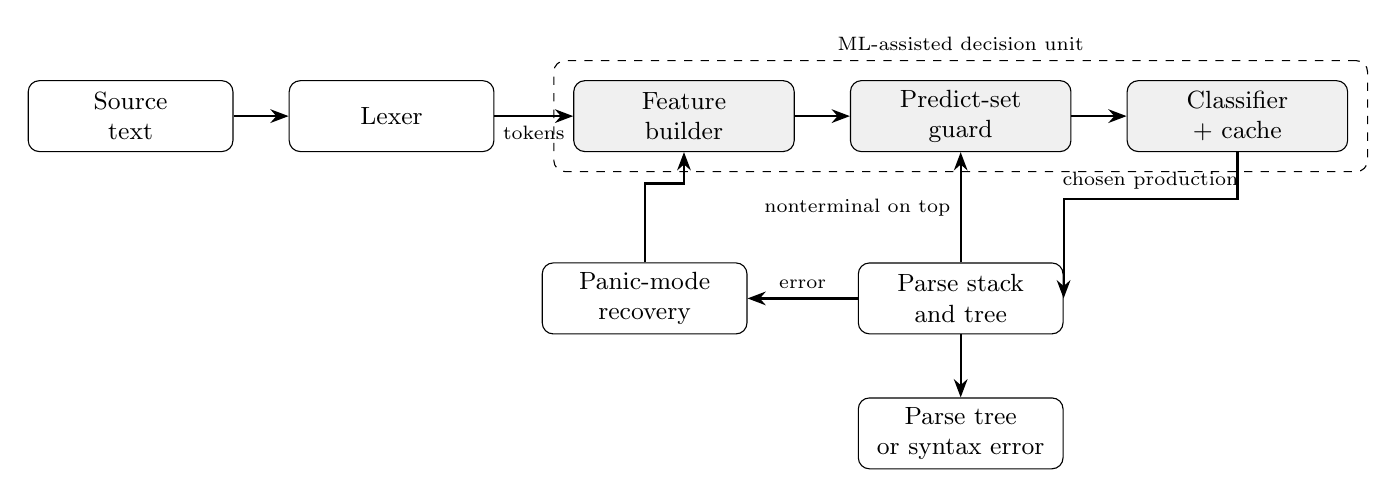
\begin{tikzpicture}[
  node distance=0.7cm,
  box/.style={rectangle,rounded corners,draw,minimum width=2.6cm,minimum height=0.9cm,align=center,font=\small},
  sbox/.style={rectangle,rounded corners,draw,fill=gray!12,minimum width=2.8cm,minimum height=0.9cm,align=center,font=\small},
  arrow/.style={-{Stealth},thick}]
\node[box] (src) {Source\\text};
\node[box,right=of src] (lex) {Lexer};
\node[sbox,right=1.0cm of lex] (feat) {Feature\\builder};
\node[sbox,right=of feat] (guard) {Predict-set\\guard};
\node[sbox,right=of guard] (ml) {Classifier\\+ cache};
\node[box,below=1.4cm of guard] (stack) {Parse stack\\and tree};
\node[box,below=0.8cm of stack] (out) {Parse tree\\or syntax error};
\node[box,left=1.4cm of stack] (rec) {Panic-mode\\recovery};
\draw[arrow] (src)--(lex);
\draw[arrow] (lex) -- node[below,font=\scriptsize]{tokens} (feat);
\draw[arrow] (feat)--(guard);
\draw[arrow] (guard)--(ml);
\draw[arrow] (ml.south) -- ++(0,-0.6) -| node[pos=0.25,above,font=\scriptsize]{chosen production} (stack.east);
\draw[arrow] (stack.north) -- node[left,font=\scriptsize]{nonterminal on top} (guard.south);
\draw[arrow] (stack) -- (out);
\draw[arrow] (stack) -- node[above,font=\scriptsize]{error} (rec);
\draw[arrow] (rec.north) |- ++(0,1.0) -| (feat.south);
\begin{scope}[on background layer]
\node[draw,dashed,rounded corners,fit=(feat)(guard)(ml),inner sep=7pt,label={[font=\scriptsize]above:ML-assisted decision unit}] {};
\end{scope}
\end{tikzpicture}}
\caption{Run-time architecture of the ML-based predictive parser. The shaded blocks form the decision unit that replaces the parse-table lookup.}
\label{fig:arch}
\end{figure}

\begin{figure}[H]
\centering
\resizebox{\textwidth}{!}{%
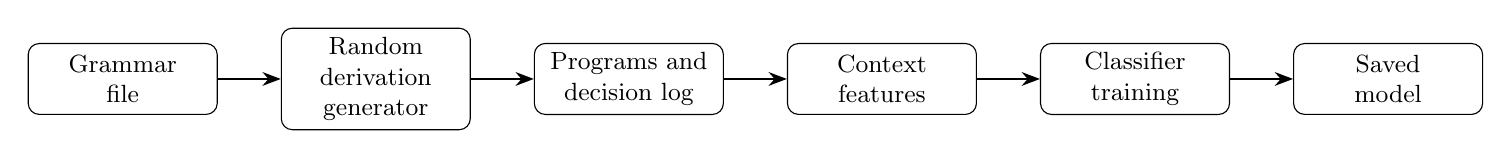
\begin{tikzpicture}[
  node distance=0.8cm,
  box/.style={rectangle,rounded corners,draw,minimum width=2.4cm,minimum height=0.9cm,align=center,font=\small},
  arrow/.style={-{Stealth},thick}]
\node[box] (g) {Grammar\\file};
\node[box,right=of g] (gen) {Random\\derivation\\generator};
\node[box,right=of gen] (ds) {Programs and\\decision log};
\node[box,right=of ds] (fe) {Context\\features};
\node[box,right=of fe] (tr) {Classifier\\training};
\node[box,right=of tr] (mod) {Saved\\model};
\foreach \a/\b in {g/gen,gen/ds,ds/fe,fe/tr,tr/mod} \draw[arrow] (\a)--(\b);
\end{tikzpicture}}
\caption{Offline pipeline: labelled decisions are harvested directly from derivations.}
\label{fig:train}
\end{figure}

\subsection{Feature Design}

Each decision is described by eight categorical features computed from the
token stream (Table~\ref{tab:features}). Three nested feature sets are used for
ablation: F1 uses the first two, F2 adds the second lookahead, and F3 uses all
eight.

\begin{table}[H]
\centering
\caption{Decision-context features.}
\label{tab:features}
\small
\begin{tabularx}{\textwidth}{llX}
\toprule
\textbf{Feature} & \textbf{Set} & \textbf{Meaning}\\
\midrule
\texttt{nt}     & F1 & Nonterminal being expanded\\
\texttt{la1}    & F1 & First lookahead token\\
\texttt{la2}    & F2 & Second lookahead token\\
\texttt{la3}    & F3 & Third lookahead token\\
\texttt{prev}   & F3 & Previously consumed token\\
\texttt{parent} & F3 & Nonterminal whose production introduced this one\\
\texttt{brace}  & F3 & Current brace nesting depth (capped at 4)\\
\texttt{paren}  & F3 & Current parenthesis nesting depth (capped at 4)\\
\bottomrule
\end{tabularx}
\end{table}

\subsection{Training-Data Generation}

No manually annotated treebank is needed. The generator performs a random
leftmost derivation: at each nonterminal it samples one production, with a
tunable bias toward the empty alternative that controls program length, and it
forces the cheapest production once a depth or length limit is exceeded so that
every derivation terminates. The generator logs the nonterminal, the chosen
production, the token position and the parent. After the sentence is complete
the features are computed from the finished token stream. The labels are
therefore the true derivation choices. Section~5.5 reports two checks
that validate this: for the LL(1) grammar the logged decisions are identical to
those of the classical parser, and for the extended grammar the triple
$(A,a_1,a_2)$ determines the production without exception.

\subsection{Pure and Guarded Decision Modes}

\paragraph{Pure mode.} The classifier outputs a probability for every
production in the grammar. We take the most probable production among those
whose left-hand side equals the current nonterminal $A$.

\paragraph{Guarded mode.} Let
\begin{equation}
C(A,a)=\{\,p=(A\rightarrow\alpha)\;:\;a\in\mathrm{PS}(p)\,\}
\end{equation}
be the set of productions whose predict set (Eq.~\ref{eq:ps}) contains the first
lookahead $a$. The parser then acts as follows:
\begin{itemize}
    \item $|C|=0$: no production can start with the lookahead, so a syntax error is reported at this token;
    \item $|C|=1$: the single candidate is taken and the model is not consulted;
    \item $|C|\ge 2$: this is an LL(1) conflict, and the classifier picks
    $\arg\max_{p\in C}P_\theta(p\mid\mathbf{x})$.
\end{itemize}
Guarded mode therefore uses the grammar for everything the grammar can decide
and the model only where the grammar is genuinely undecided. It was introduced
after pure mode exhibited the soundness problem described in
Section~7.6.

\subsection{Algorithm}

\begin{algorithm}[H]
\caption{ML-assisted predictive parsing (guarded mode)}
\label{alg:mlparse}
\begin{algorithmic}[1]
\Require Token list $w$, grammar $G$, trained model $f_\theta$, predict sets $\mathrm{PS}$
\Ensure Parse tree, or a syntax error with its position
\State $stack \gets [\$,\;S]$; \quad $i \gets 0$
\While{$stack$ not empty}
  \State $X \gets \textsc{Pop}(stack)$; \quad $a \gets w[i]$
  \If{$X$ is a nonterminal}
     \State $C \gets \{p : \mathrm{lhs}(p)=X,\; a\in\mathrm{PS}(p)\}$
     \If{$C=\emptyset$} \State \Return \textsc{SyntaxError}$(i)$ \EndIf
     \If{$|C|=1$} \State $p \gets$ the only element of $C$
     \Else \State $\mathbf{x} \gets \textsc{Features}(X,w,i,\ldots)$; \quad $p \gets \arg\max_{q\in C} P_\theta(q\mid\mathbf{x})$ \EndIf
     \State push $\mathrm{rhs}(p)$ onto $stack$ in reverse order; attach children to the tree
  \ElsIf{$X=a$}
     \If{$X=\$$} \State \Return the tree \EndIf
     \State $i \gets i+1$
  \Else
     \State \Return \textsc{SyntaxError}$(i)$
  \EndIf
\EndWhile
\end{algorithmic}
\end{algorithm}

\subsection{Error Detection and Panic-Mode Recovery}

An error arises when a nonterminal has no admissible production or when the
expected terminal differs from the lookahead. Without recovery the parser stops
and reports the token index. With recovery enabled it applies panic mode:
input is discarded up to the next statement terminator (\tok{;}) or closing
brace, the stack is unwound to the nearest \ntm{StmtList} or closing brace, and
parsing resumes, so that later errors in the same program can still be found.
A step counter protects against non-terminating expansions.

\subsection{Prediction Cache}

A decision is fully determined by the feature tuple (and the candidate set), so
the result can be memoised. During a run, identical contexts recur often, and
the cache converts most classifier invocations into dictionary lookups. The
cache is the difference between an unusable and a practical parser, as
Section~7.10 shows.

\subsection{Adapting to a Changed Grammar}

When the language gains a construct, a classical generator must recompute its
tables, and if the new construct creates conflicts, a person must rewrite
rules. The ML parser is instead retrained: samples of programs using the new
construct are generated or collected, merged with the existing training data
(productions are identified by their textual form so that labels survive the
change of grammar), and the model is refitted. Section~7.9 measures how many
new programs are required.

\newpage
% ============================================================
% 5. IMPLEMENTATION
% ============================================================
\section{Implementation}

\subsection{Environment}

\begin{table}[H]
\centering
\caption{Software environment used for all experiments.}
\label{tab:env}
\begin{tabular}{ll}
\toprule
\textbf{Component} & \textbf{Detail}\\
\midrule
Language & Python 3.12\\
Machine-learning library & scikit-learn 1.8.0\\
Numerical / data libraries & NumPy 2.4, pandas\\
Plotting & Matplotlib 3.10\\
Execution & Single thread, pure Python parsers\\
Report typesetting & \LaTeX{} (pdflatex)\\
\bottomrule
\end{tabular}
\end{table}

Python was chosen because it allows the grammar toolkit, the parsers and the
learning code to live in a single language and be tested together.

\subsection{Project Structure}

\begin{table}[H]
\centering
\caption{Source files of the implementation.}
\label{tab:files}
\small
\begin{tabularx}{\textwidth}{lX}
\toprule
\textbf{File} & \textbf{Purpose}\\
\midrule
\texttt{grammar.py} & Reads grammar files; computes FIRST, FOLLOW, LL(1) table and conflicts\\
\texttt{lexer.py} & Regular-expression tokenizer for the mini language\\
\texttt{ll1\_parser.py} & Table-driven LL(1) predictive parser; logs every decision\\
\texttt{slr\_parser.py} & SLR(1) item sets, ACTION/GOTO tables, shift-reduce parser\\
\texttt{generator.py} & Random derivation generator and feature extraction\\
\texttt{train\_part2.py} & Dataset creation and model training/evaluation\\
\texttt{oracle.py} & Exhaustive backtracking recognizer used as ground truth\\
\texttt{ml\_parser.py} & ML-based predictive parser (pure and guarded), recovery, cache\\
\texttt{part3\_exp1.py}, \texttt{part3\_exp2.py} & End-to-end, error, speed, learning and adaptation experiments\\
\texttt{make\_figures.py} & Produces the plots used in this report\\
\texttt{grammars/*.txt} & The three grammar files (G1 for LL, G1 for LR, G2)\\
\bottomrule
\end{tabularx}
\end{table}

\subsection{The Grammars}

The test language is a small imperative language with assignment, \tok{if}/\tok{else},
\tok{while}, \tok{print}, arithmetic with the usual precedence, and relational
conditions. Two versions were used.

\paragraph{G1.} The conflict-free version, written in LL(1) form (right-recursive
expression rules). A left-recursive version of the same language is used for the
SLR(1) parser.

\paragraph{G2.} G1 extended with function calls: a statement such as
\tok{f(a, 1+2);} and an expression factor such as \tok{f(3)}. Both new rules begin
with an identifier, which creates two LL(1) conflicts, one on \ntm{Stmt} and one
on \ntm{Factor}, in each case for the lookahead \tok{id}. The full grammars are
listed in Appendix~A.

\begin{table}[H]
\centering
\caption{Grammar statistics.}
\label{tab:grammars}
\begin{tabular}{lrr}
\toprule
\textbf{Property} & \textbf{G1} & \textbf{G2}\\
\midrule
Productions & 25 & 31\\
Nonterminals & 11 & 13\\
Terminals & 20 & 21\\
LL(1) & Yes & No\\
Conflicting table cells & 0 & 2\\
Resolved with lookahead 2 & -- & Yes (no ambiguous context)\\
\bottomrule
\end{tabular}
\end{table}

\noindent For the left-recursive version of G1, the SLR(1) construction yields 54
automaton states and 248 ACTION entries with no conflicts.

\subsection{Key Code Excerpts}

In all listings the empty string is written \texttt{eps} for typesetting reasons.

\begin{lstlisting}[caption={Predict sets, computed once when the parser is created (ml\_parser.py).}]
self.pset = []
for lhs, rhs in grammar.productions:
    fs = grammar.first_of_seq(rhs)
    ps = fs - {"eps"}
    if "eps" in fs:
        ps |= grammar.follow[lhs]
    self.pset.append(ps)
\end{lstlisting}

\begin{lstlisting}[caption={The decision procedure of the guarded parser (ml\_parser.py).}]
def choose(self, feat):
    nt, la = feat["nt"], feat["la1"]
    if self.mode == "guarded":
        cands = self.candidates(nt, la)   # productions whose predict set holds la
        if not cands:
            return None                   # syntax error
        if len(cands) == 1:
            return cands[0]               # grammar decides; no model call
        return self._ml_choose(feat, cands)
    return self._ml_choose(feat, self.g.by_lhs[nt])
\end{lstlisting}

\begin{lstlisting}[caption={Random leftmost derivation that records labelled decisions (generator.py).}]
def _expand(self, nt, depth, parent, toks, ev):
    cands = self.g.by_lhs[nt]
    if depth > self.max_depth or len(toks) > self.max_tokens:
        pi = min(cands, key=self._prod_cost)      # force termination
    else:
        w = [EPS_WEIGHT.get(nt, 1.0) if not self.g.productions[i][1] else 1.0
             for i in cands]
        pi = self.rng.choices(cands, weights=w)[0]
    ev.append({"nt": nt, "prod": pi, "pos": len(toks), "parent": parent})
    for s in self.g.productions[pi][1]:
        if self.g.is_nt(s):
            self._expand(s, depth + 1, nt, toks, ev)
        else:
            toks.append(s)
\end{lstlisting}

\begin{lstlisting}[caption={Exact reference recognizer returning validity and the longest viable prefix (oracle.py).}]
def rec(stack, pos):
    key = (stack, pos)
    if key in seen:
        return False
    seen.add(key)
    best[0] = max(best[0], pos)               # furthest token matched so far
    if not stack:
        return pos == n
    s, rest = stack[0], stack[1:]
    if g.is_nt(s):
        return any(rec(g.productions[pi][1] + rest, pos) for pi in g.by_lhs[s])
    return pos < n and toks[pos] == s and rec(rest, pos + 1)
\end{lstlisting}

\subsection{Validation of the Data and Components}

Before any learning result is trusted, three checks were run.

\begin{enumerate}
    \item \textbf{Parsers agree.} The LL(1) and SLR(1) parsers return the same
    accept/reject verdict on five valid and eight invalid programs
    (Table~\ref{tab:accept}).
    \item \textbf{Generator labels are correct.} On 300 programs of G1, the
    decisions logged by the generator are identical to the decisions made by the
    classical LL(1) parser.
    \item \textbf{A perfect answer exists for G2.} Over 2,000 generated programs,
    the triple (nonterminal, first lookahead, second lookahead) maps to exactly
    one production in every case, so the conflicts are resolvable with two
    tokens of lookahead and the learning task is well posed.
\end{enumerate}

\newpage
% ============================================================
% 6. EXPERIMENTAL SETUP
% ============================================================
\section{Experimental Setup}

\subsection{Datasets}

For each grammar, 2,500 random programs were generated and every parsing
decision was logged. The first 2,000 programs form the training set and the
remaining 500 the test set, so that no program contributes to both. All
decisions of a program stay on the same side of the split.

\begin{table}[H]
\centering
\caption{Generated datasets.}
\label{tab:data}
\begin{tabular}{lrr}
\toprule
\textbf{Quantity} & \textbf{G1} & \textbf{G2}\\
\midrule
Programs & 2,500 & 2,500\\
Average tokens per program & 74.3 & 72.5\\
Parsing decisions (total) & 319,980 & 305,142\\
Training decisions (2,000 programs) & 258,187 & 245,889\\
Test decisions (500 programs) & 61,793 & 59,253\\
\bottomrule
\end{tabular}
\end{table}

Later experiments use fresh programs generated with different random seeds:
400 valid programs per grammar for end-to-end parsing, 600 single-token
mutations per grammar for error tests, and 200 programs with up to three
injected errors for recovery.

\subsection{Evaluation Metrics}

\begin{itemize}
    \item \textbf{Decision accuracy} is the fraction of individual parsing
    decisions for which the predicted production equals the true one.
    \item \textbf{Program accuracy} is the fraction of programs for which
    \emph{every} decision is correct. This is the metric that matters for
    parsing, since one wrong choice usually breaks the parse.
    \item \textbf{Conflict accuracy} is decision accuracy restricted to the
    decisions where the LL(1) table is ambiguous (nonterminal \ntm{Stmt} or
    \ntm{Factor} with lookahead \tok{id}).
    \item \textbf{Agreement with the oracle}, \textbf{false accepts} (invalid
    programs accepted) and \textbf{false rejects} (valid programs rejected).
    \item \textbf{Exact error position}: for an invalid program let $k^{*}$ be
    the length of the longest prefix that can still be extended to a valid
    program, as computed by the oracle. A parser reports the error at the exact
    position when it stops at token index $k^{*}$.
    \item \textbf{Time per program} (ms) and throughput (tokens per second).
\end{itemize}

\subsection{Experimental Protocol}

\begin{enumerate}
    \item Compare the classical LL(1) table with the learned models on the
    held-out decisions (Section~7.2), including a feature ablation (7.3).
    \item Measure the learning curve (7.4).
    \item Run complete parses on fresh valid programs (7.5).
    \item Test error detection and localisation on mutated programs (7.6)
    and recovery (7.7).
    \item Test generalisation to much longer programs (7.8).
    \item Test adaptation from G1 to G2 (7.9).
    \item Measure running time (7.10).
\end{enumerate}

Random seeds are fixed in all scripts, so each experiment is repeatable.

\newpage
% ============================================================
% 7. RESULTS AND DISCUSSION
% ============================================================
\section{Results and Discussion}

\subsection{Baseline Parsers}

The LL(1) table of G1 has 56 non-empty cells, and G1 is conflict-free. The SLR(1)
automaton of the left-recursive variant has 54 states. Table~\ref{tab:accept}
lists the verdicts on a small acceptance suite; both parsers agree with the
expected answer in all 13 cases, including the empty program.

\begin{table}[H]
\centering
\caption{Acceptance suite (LL(1) and SLR(1) give identical verdicts).}
\label{tab:accept}
\small
\begin{tabular}{llc}
\toprule
\textbf{Program} & \textbf{Expected} & \textbf{LL / SLR}\\
\midrule
\tok{x = 1 + 2 * 3;} & valid & accept / accept\\
\tok{a = (b + c) * d - 4 / e;} & valid & accept / accept\\
\tok{if (x < 10) \{ y = x + 1; \} else \{ y = 0; \}} & valid & accept / accept\\
\tok{while (i != 5) \{ print(i); i = i + 1; \}} & valid & accept / accept\\
(empty program) & valid & accept / accept\\
\tok{x = ;} \quad \tok{x = 1 + ;} \quad \tok{if (x < ) \{ \}} & invalid & reject / reject\\
\tok{while x < 3 \{ \}} \quad \tok{x = (1 + 2;} & invalid & reject / reject\\
\tok{print(x)} \quad \tok{else \{ \}} \quad \tok{x = 1 2;} & invalid & reject / reject\\
\bottomrule
\end{tabular}
\end{table}

\subsection{Decision and Program Accuracy}

Table~\ref{tab:acc} and Figure~\ref{fig:acc} compare the classical table with
the learned models on the held-out test decisions.

\begin{table}[H]
\centering
\caption{Accuracy on the held-out test programs (500 per grammar). DT = decision tree; F1/F2/F3 are the feature sets of Table~\ref{tab:features}.}
\label{tab:acc}
\footnotesize
\resizebox{\textwidth}{!}{%
\begin{tabular}{llrrrr}
\toprule
\textbf{Grammar} & \textbf{Method} & \textbf{Decision (\%)} & \textbf{Program (\%)} & \textbf{Train (s)} & \textbf{Infer. ($\mu$s/dec.)}\\
\midrule
G1 & Classical LL(1) table & 100.0 & 100.0 & -- & --\\
G1 & DT, F1 / F2 / F3 & 100.0 & 100.0 & 0.3 / 0.3 / 0.9 & 1.8 / 1.4 / 1.8\\
G1 & Random forest, F3 & 100.0 & 100.0 & 12.1 & 5.5\\
G1 & MLP, F3 & 100.0 & 100.0 & 13.8 & 3.7\\
\midrule
G2 & Classical table (first rule wins) & 89.5 & 45.4 & -- & --\\
G2 & DT, F1 & 95.1 & 49.2 & 0.2 & 1.8\\
G2 & DT, F2 & 100.0 & 100.0 & 0.3 & 1.9\\
G2 & DT, F3 & 100.0 & 100.0 & 0.7 & 2.0\\
G2 & Random forest, F3 & 100.0 & 100.0 & 14.1 & 5.5\\
G2 & MLP, F3 & 100.0 & 100.0 & 16.2 & 2.8\\
\bottomrule
\end{tabular}}
\end{table}

\begin{figure}[H]
\centering
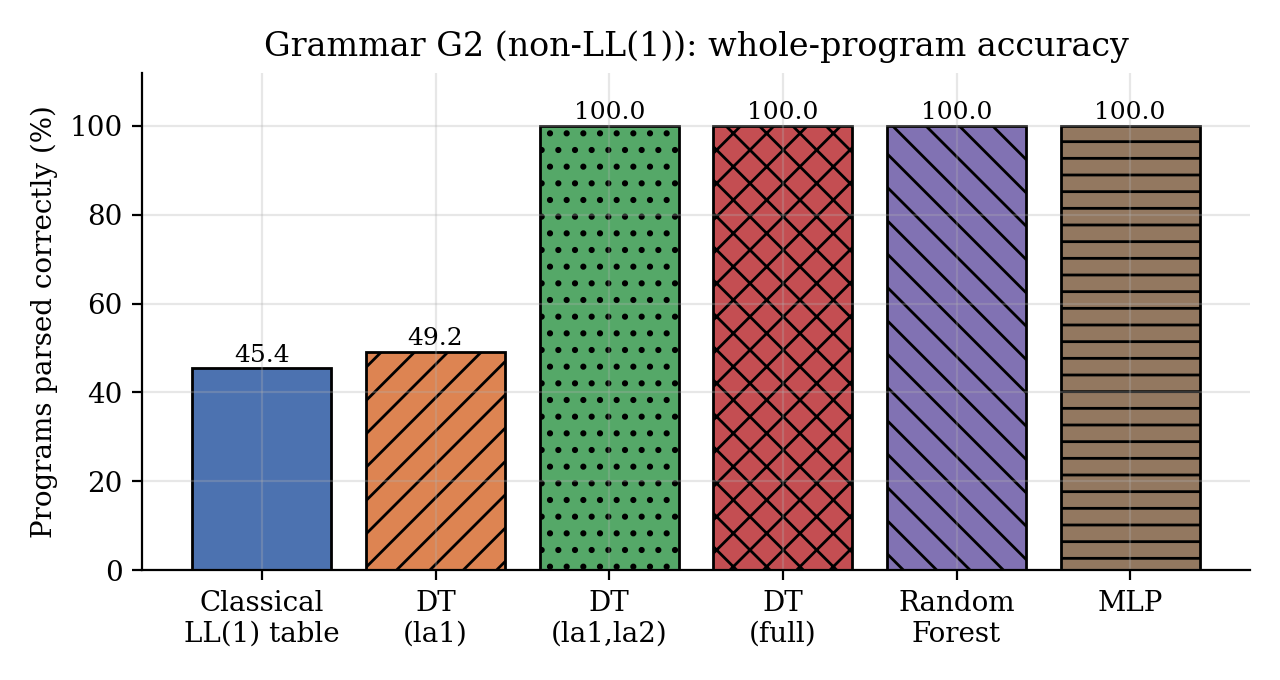
\includegraphics[width=0.82\textwidth]{figures/fig_accuracy_g2.png}
\caption{Whole-program accuracy on the non-LL(1) grammar G2.}
\label{fig:acc}
\end{figure}

On G1 there is nothing for a model to add: the pair (nonterminal, lookahead)
already determines the rule, and all methods are perfect, as expected. On G2 the
picture changes sharply. When the classical table is forced to keep one rule in
each conflicting cell, it makes about 10.5\% of the decisions wrongly
(6,125 on \ntm{Factor} and 77 on \ntm{Stmt}, out of 59,253), and since a single
wrong decision ruins a parse, only 45.4\% of programs are handled correctly.
The one-lookahead decision tree is better at the decision level because it picks
the majority rule per context, but it cannot exceed 49.2\% at the program level.
The decision trees given the second lookahead token, the random forest and the
MLP are all perfect.

\subsection{Which Context Matters}

Retraining a decision tree on only the conflict decisions and summing the
importances of the one-hot columns that belong to each feature gives
Figure~\ref{fig:imp}. The second lookahead token accounts for 93.6\% of the
learned importance, the parent nonterminal for 3.3\% and the nonterminal itself
for 3.1\%; the remaining features score zero.

\begin{figure}[H]
\centering
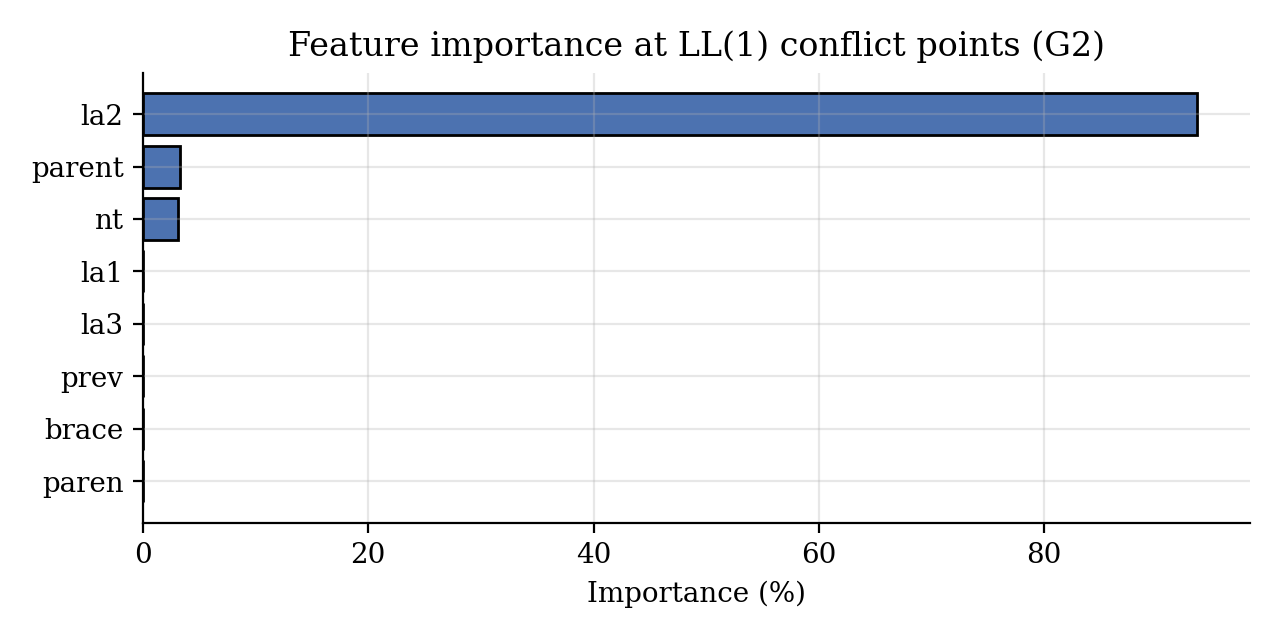
\includegraphics[width=0.78\textwidth]{figures/fig_importance.png}
\caption{Feature importance at the LL(1) conflict points of G2.}
\label{fig:imp}
\end{figure}

This is the pattern one would predict by reading the grammar: the two competing
statement rules differ in whether \tok{=} or \tok{(} follows the identifier, and the
two factor rules in whether \tok{(} follows. The model has therefore rediscovered
the LL(2) rule on its own, which is a useful sanity check on what it learned,
and it explains why the extra features of F3 make no difference to accuracy.

\subsection{Learning Curve}

\begin{table}[H]
\centering
\caption{Program accuracy (\%) on G2 as the number of training programs grows.}
\label{tab:lc}
\begin{tabular}{rrrrrr}
\toprule
\textbf{Programs} & \textbf{Decisions} & \textbf{DT, F1} & \textbf{DT, F2} & \textbf{DT, F3} & \textbf{MLP, F3}\\
\midrule
5    & 500     & 47.8 & 53.8 & 50.6 & 44.6\\
10   & 990     & 47.8 & 60.2 & 58.0 & 47.2\\
25   & 2,749   & 47.8 & 79.4 & 76.2 & 81.4\\
50   & 5,781   & 49.2 & 91.6 & 88.6 & 97.2\\
100  & 12,395  & 49.2 & 99.8 & 99.4 & 99.4\\
250  & 30,517  & 49.2 & 99.8 & 99.8 & 99.6\\
500  & 58,290  & 49.2 & 100.0 & 100.0 & 100.0\\
2,000& 245,889 & 49.2 & 100.0 & 100.0 & 100.0\\
\bottomrule
\end{tabular}
\end{table}

\begin{figure}[H]
\centering
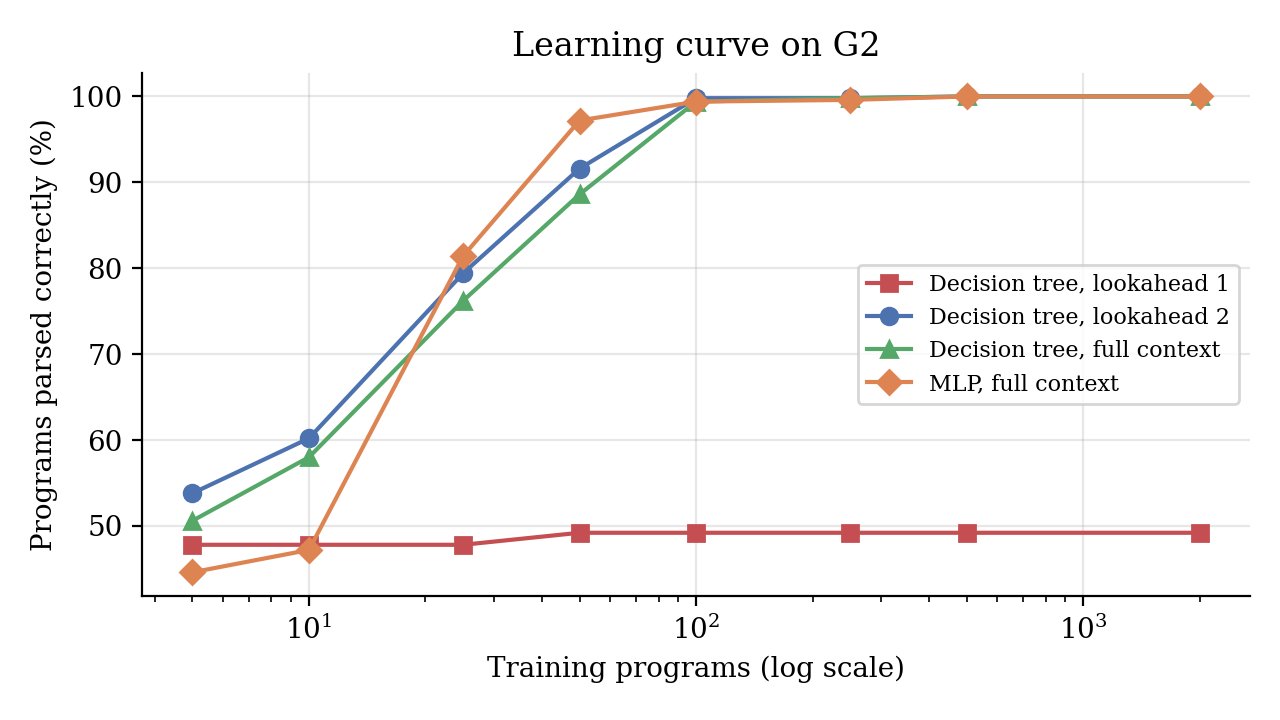
\includegraphics[width=0.82\textwidth]{figures/fig_learning_curve.png}
\caption{Program accuracy on G2 versus the number of training programs.}
\label{fig:lc}
\end{figure}

Around one hundred programs (about 12,000 decisions) bring every model with
the second lookahead within a fraction of a percent of perfection. The
lookahead-1 tree never improves, because additional data cannot supply the
missing information. Note that the F2 tree already makes the conflict decisions
correctly 99.3\% of the time with only five programs; the program-level curve
rises more slowly because, in pure mode, the model also has to learn all the
non-conflict decisions from the same data.

\subsection{End-to-End Parsing of Valid Programs}

The models were then embedded in the full parser and run on 400 fresh valid
programs per grammar (Table~\ref{tab:e2e}). On G1 the ML parser builds a parse
tree identical to the classical tree in all 400 programs. On G2 the classical
parser with first-rule-wins resolution parses 43.3\% of the programs; both ML
modes parse all of them.

\begin{table}[H]
\centering
\caption{Valid programs accepted in end-to-end parsing (400 per grammar).}
\label{tab:e2e}
\begin{tabular}{lrr}
\toprule
\textbf{Parser} & \textbf{G1 (\%)} & \textbf{G2 (\%)}\\
\midrule
Classical LL(1) (first rule wins on conflicts) & 100.0 & 43.3\\
ML parser, pure mode & 100.0 & 100.0\\
ML parser, guarded mode & 100.0 & 100.0\\
\bottomrule
\end{tabular}
\end{table}

\subsection{Error Detection and Localisation}

Each grammar was tested with 600 mutants made by deleting, inserting or
replacing one token of a valid program (584 mutants of G1 and 577 of G2 turned
out invalid; the others happened to be valid). The oracle supplies the true
verdict and the true error position $k^{*}$.

\begin{table}[H]
\centering
\caption{Error detection on 600 mutated programs per grammar, after correcting the termination defect.}
\label{tab:err}
\small
\begin{tabular}{llrrrr}
\toprule
\textbf{Grammar} & \textbf{Parser} & \textbf{Agreement (\%)} & \textbf{False acc.} & \textbf{False rej.} & \textbf{Exact pos. (\%)}\\
\midrule
G1 & Classical LL(1) & 100.0 & 0 & 0 & 100.0\\
G1 & ML pure & 100.0 & 0 & 0 & 86.3\\
G1 & ML guarded & 100.0 & 0 & 0 & 100.0\\
\midrule
G2 & Classical (first wins) & 96.8 & 0 & 19 & 48.4\\
G2 & ML pure & 100.0 & 0 & 0 & 92.0\\
G2 & ML guarded & 100.0 & 0 & 0 & 100.0\\
\bottomrule
\end{tabular}
\end{table}

\begin{figure}[H]
\centering
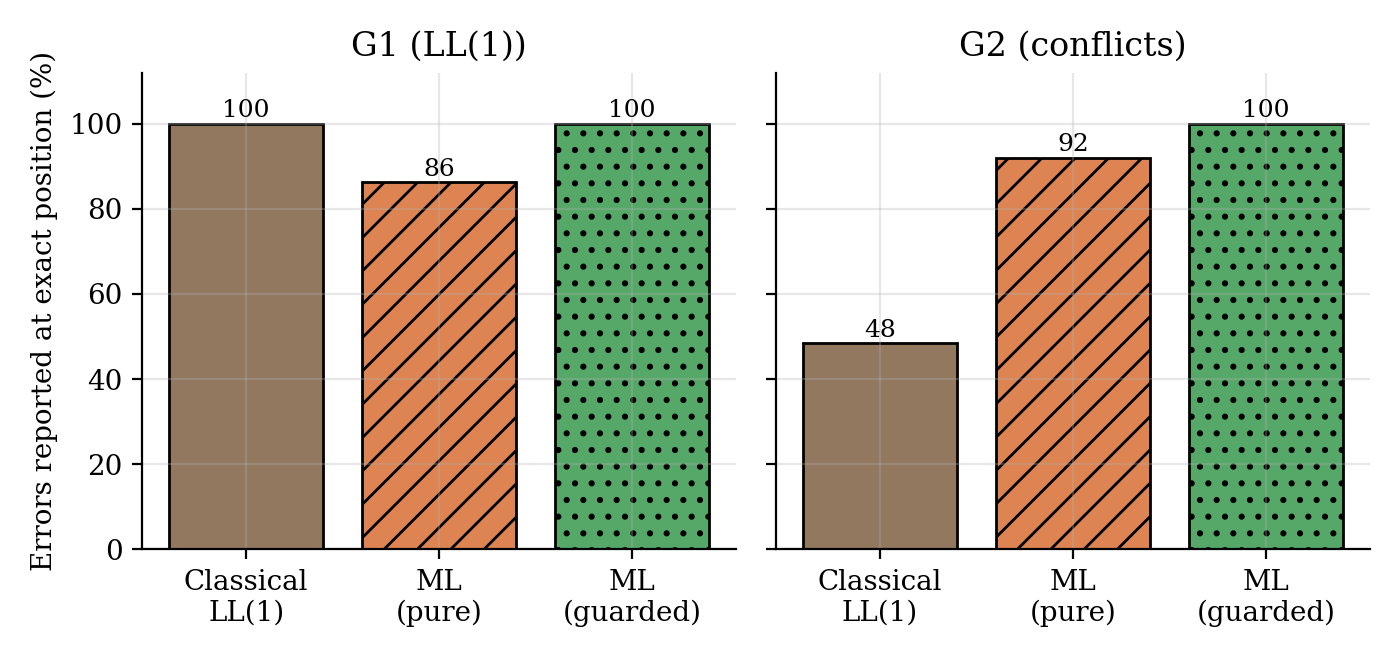
\includegraphics[width=0.85\textwidth]{figures/fig_error_localisation.png}
\caption{Share of syntax errors reported at exactly the oracle position.}
\label{fig:loc}
\end{figure}

\paragraph{A defect found along the way.} In the first version of the pure-ML
parser, 70 of 600 invalid mutants of G1 (88.3\% agreement) and 31 of 600 of G2
(94.8\% agreement) were wrongly accepted. The cause was not the model's
accuracy but a missing safeguard. On an invalid input the model meets contexts
it never saw and can keep predicting a recursive production, so the parse never
reaches the end; a step limit added to prevent infinite loops then ended
the loop and, because it did not raise an error in non-recovery mode, the
parser returned success. Two changes removed the defect: hitting the limit now
raises a syntax error, and the guarded mode forbids any production whose predict
set excludes the lookahead. After the fix no false acceptances remain.

\paragraph{Interpretation.} In guarded mode every error is reported at exactly
the oracle position, as in the classical parser on G1, because the guard
detects an impossible lookahead at the same moment the table would find an empty
cell. Pure mode finds all errors but sometimes later than necessary (86.3\% and
92.0\% exact), since a wrongly predicted rule can consume a few more tokens
before the mismatch appears. The classical parser on G2 is the worst case: it
rejects 19 valid mutants outright, and when it correctly rejects, it points at
the right token only 48.4\% of the time, because it has already committed to a
wrong rule at an earlier conflict.

\subsection{Error Recovery}

Two hundred programs of 25--80 tokens were each given one to three random
token substitutions (400 injected errors in total) and parsed with panic-mode
recovery on.

\begin{table}[H]
\centering
\caption{Panic-mode recovery on G2 (200 programs, 400 injected errors).}
\label{tab:rec}
\begin{tabular}{lrr}
\toprule
\textbf{Quantity} & \textbf{Pure} & \textbf{Guarded}\\
\midrule
Programs parsed without crashing & 200 & 200\\
Programs with at least one error reported & 200 & 200\\
Errors reported & 286 & 253\\
Programs with no error reported at the very end of input & 172 & 196\\
\bottomrule
\end{tabular}
\end{table}

Recovery was robust in both modes: it never crashed or looped, and every faulty
program was flagged. The guarded mode resynchronised better, with 196 of 200
programs not ending in a spurious end-of-input error against 172 for pure mode.
The number of reported errors is lower than the number injected because panic
mode skips to the next statement boundary, so two errors in one statement count
once, and because some substitutions produce another legal token. The count is
thus not a precision measure of recovery quality, only an indication that
recovery continues past the first error.

\subsection{Generalisation to Longer Programs}

Models were trained on short programs (about 35 decisions on average) and tested
on much longer ones (150 programs of at least 100 tokens, about 671 decisions on
average).

\begin{table}[H]
\centering
\caption{Training on short programs and testing on long ones (G2).}
\label{tab:len}
\resizebox{\textwidth}{!}{%
\begin{tabular}{lrrrrr}
\toprule
\textbf{Model} & \textbf{Short: dec. (\%)} & \textbf{Short: prog. (\%)} & \textbf{Long: dec. (\%)} & \textbf{Long: prog. (\%)} & \textbf{Long: conflict (\%)}\\
\midrule
DT, F2   & 100 & 100 & 99.997 & 98.0 & 100\\
DT, F3   & 100 & 100 & 99.997 & 98.0 & 100\\
MLP, F3  & 100 & 100 & 99.997 & 98.0 & 100\\
\bottomrule
\end{tabular}}
\end{table}

Even on programs nearly twenty times longer than those seen in training,
the models misjudge only a handful of decisions (three of 150 programs fail),
and none of them at a conflict point. The failures are therefore non-conflict
decisions, which the pure mode must predict but the guarded mode takes from the
grammar. We expect the guarded parser to be unaffected, since its only learned
decisions are the conflict ones, but this was derived from the conflict
accuracy rather than measured separately.

\subsection{Adapting to a Changed Grammar}

A decision tree trained only on G1 data was applied to G2. Programs
using function calls were then progressively added to the G1 training set and
the model was retrained from scratch. Productions were identified by their
textual form so that labels transfer between grammars.

\begin{table}[H]
\centering
\caption{Adapting a G1-trained model to G2 by adding new-grammar programs (test: 500 G2 programs).}
\label{tab:adapt}
\begin{tabular}{rrrrr}
\toprule
\textbf{New programs} & \textbf{Decision (\%)} & \textbf{Conflict (\%)} & \textbf{Program (\%)} & \textbf{Retrain (s)}\\
\midrule
0   & 87.0  & 67.9  & 46.4  & 1.29\\
5   & 99.9  & 99.6  & 92.0  & 1.30\\
10  & 100.0 & 100.0 & 100.0 & 1.20\\
25  & 100.0 & 100.0 & 100.0 & 1.10\\
50  & 100.0 & 100.0 & 100.0 & 1.16\\
100 & 100.0 & 100.0 & 100.0 & 1.17\\
500 & 100.0 & 100.0 & 100.0 & 1.51\\
\bottomrule
\end{tabular}
\end{table}

\begin{figure}[H]
\centering
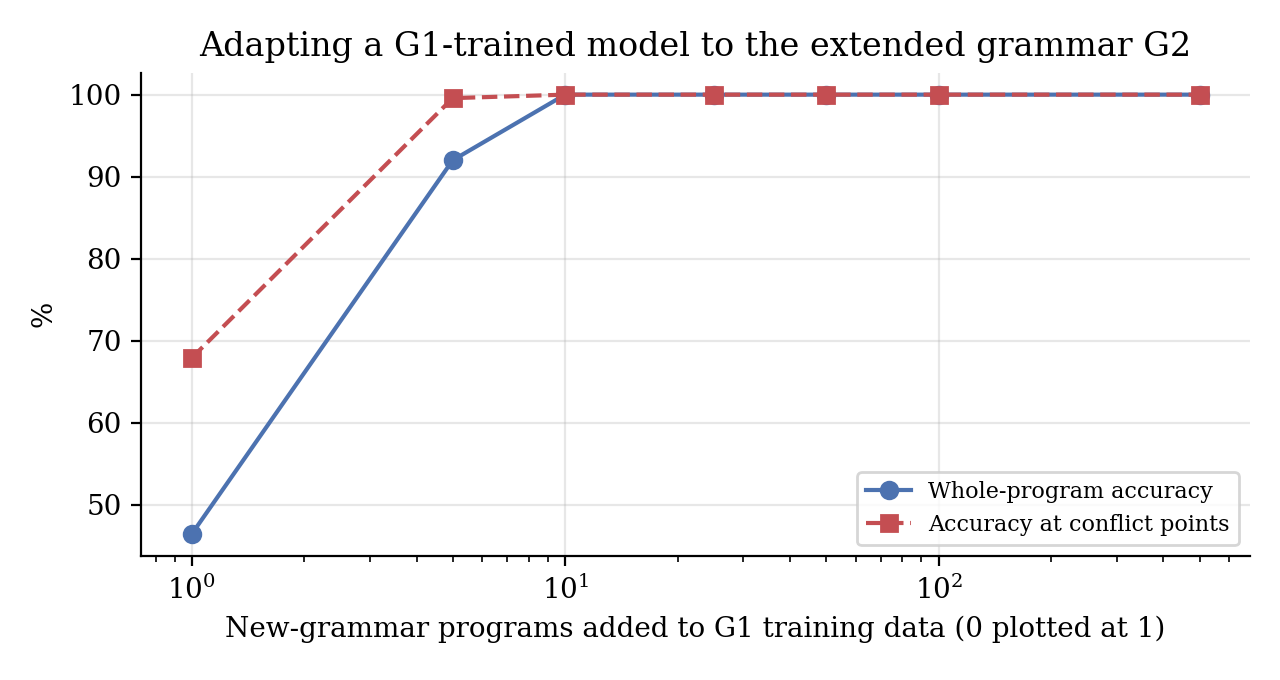
\includegraphics[width=0.82\textwidth]{figures/fig_adaptation.png}
\caption{Accuracy on G2 as new-grammar programs are added to the G1 data.}
\label{fig:adapt}
\end{figure}

Without any new data the G1 model is wrong on nearly half of the G2 programs,
because it has never seen the call productions. Five programs lift program
accuracy to 92\% and ten to 100\%, with a retraining time of about 1.2 seconds. For
comparison, recomputing the classical LL(1) table takes under a millisecond,
but for G2 the result still contains two conflicts, and removing them requires
a person to left-factor the grammar. The two approaches therefore trade human
effort against computing: the table is faster to rebuild, the model is easier
to adapt to a grammar that is no longer LL(1).

\subsection{Running Time}

Timings were taken on a single thread, as the best of three runs over 200
programs; the absolute numbers depend on the machine, so only ratios should be
read from them.

\begin{table}[H]
\centering
\caption{Parsing speed (200 programs per grammar).}
\label{tab:speed}
\small
\begin{tabular}{llrr}
\toprule
\textbf{Grammar} & \textbf{Parser} & \textbf{ms / program} & \textbf{Tokens / s}\\
\midrule
G1 & SLR(1) & 0.17 & 501,500\\
G1 & Classical LL(1) & 0.25 & 339,200\\
G1 & ML guarded (no model calls needed) & 0.48 & 179,200\\
G1 & ML pure, cached & 0.62 & 138,400\\
G1 & ML pure, no cache$^{*}$ & 561 & 152\\
\midrule
G2 & ML guarded, cached & 0.46 & 166,400\\
G2 & ML pure, cached & 0.58 & 134,000\\
G2 & ML guarded, no cache$^{*}$ & 67.5 & 1,142\\
\bottomrule
\end{tabular}

\smallskip
\footnotesize $^{*}$Measured on 30 programs and scaled to 200.
\end{table}

\begin{figure}[H]
\centering
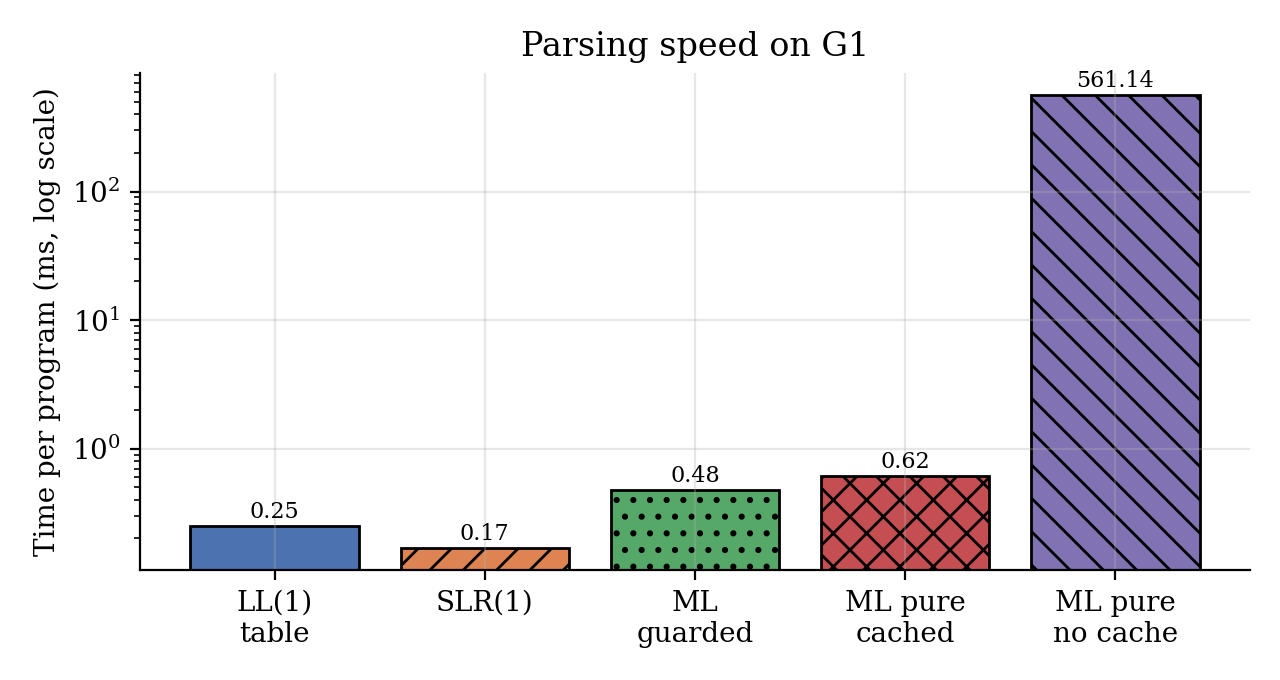
\includegraphics[width=0.82\textwidth]{figures/fig_speed.png}
\caption{Parsing time per program on G1 (logarithmic scale).}
\label{fig:speed}
\end{figure}

Three points stand out. First, the classical parsers are fastest. Second, the
cache is indispensable: the pure parser without it is more than three orders of
magnitude slower than the table, whereas with it (94.5\% hit rate on G1, 4,796
cached contexts) the slowdown falls to roughly 2.5 times. Third, the guarded
mode is cheaper than the pure mode because it never needs the model where the
grammar already decides. On G1 it made no model calls, and on G2 it needed only
469 cold model calls for 200 programs; its residual overhead over the classical
parser (about 1.9 times) comes from building the feature record at every
nonterminal expansion. Without the cache, guarded mode on G2 (67.5 ms) is also roughly eight times
faster than pure mode on G1 (561 ms), for the same reason, although these two
figures come from different grammars and are only indicative.

\subsection{Overall Discussion}

\begin{enumerate}
    \item \textbf{Where the learned parser helps.} Exactly where the classical
    table is ambiguous. It restores 100\% accuracy on a grammar where the table
    manages 43--45\%, and it needs no grammar rewriting.
    \item \textbf{Where it does not.} On an LL(1) grammar it only equals the
    table, and it costs more time.
    \item \textbf{What makes it safe.} Constraining the model by predict sets
    guarantees that it can never choose a production the grammar forbids. This
    removed all false acceptances and made error positions exact.
    \item \textbf{What makes it adaptive.} Retraining on ten new programs
    takes about a second.
    \item \textbf{What makes it fast enough.} Prediction caching, and in
    guarded mode, consulting the model only at real conflicts.
\end{enumerate}

\newpage
% ============================================================
% 8. LIMITATIONS
% ============================================================
\section{Limitations and Threats to Validity}

The results above should be read with the following caveats in mind.

\begin{itemize}
    \item \textbf{Synthetic, noise-free data.} All training and test programs
    are sampled from the same grammar by the same generator. Perfect accuracy
    on G2 partly reflects that the conflicts are cleanly resolvable by two
    tokens of lookahead. Real code, with its identifiers, comments and style,
    would be noisier, and the results do not show that the method would
    achieve the same accuracy on a full language such as C or Java.
    \item \textbf{Small grammar.} Both grammars are compact. A larger grammar
    has more decision points and conflicts that may need deeper lookahead or
    non-local context than the features used here provide.
    \item \textbf{No novelty over lookahead analysis for G2.} The conflicts in
    G2 could also be handled by an LL(2) parser or by left factoring. The point
    demonstrated is that a learned decision unit finds this solution from
    examples; the experiments do not show it beating a well-engineered
    adaptive-lookahead system such as ALL(*).
    \item \textbf{Speed.} The ML parser is slower than the table-driven
    parsers, and the measurements come from a pure-Python implementation on a
    single machine. A compiled implementation would change the absolute
    numbers, though probably not the fact that a model call is more expensive
    than a table lookup.
    \item \textbf{No formal guarantee in pure mode.} A learned model can pick
    a wrong rule on an input unlike its training data. The guarded mode
    removes the unsafe choices, but within a conflict a wrong choice among the
    allowed rules is still possible.
    \item \textbf{Mutation-based error tests.} Errors were created by
    single-token edits. Human errors are less uniform, so the exact-position
    rates should not be taken as general.
    \item \textbf{Recovery measurement.} The recovery table counts reported
    errors but does not measure whether the recovered parse tree is meaningful.
    \item \textbf{Bottom-up side.} SLR(1) was implemented as a baseline and
    validated, but the learned model was applied to the top-down parser only.
\end{itemize}

% ============================================================
% 9. CONCLUSION
% ============================================================
\section{Conclusion and Future Work}

\subsection{Conclusion}

This project built and evaluated a predictive parser whose rule-selection step
is learned rather than tabulated. A conventional LL(1) table decides from one
lookahead token and therefore breaks when two alternatives begin the same way.
By describing each parsing decision with a handful of context features and
training a classifier on decisions harvested from generated programs, the
parser resolved the conflicts of an extended grammar that defeats the table.
On that grammar the classical table parsed 43\% of valid programs, while the
decision tree, random forest and neural network parsers parsed all of them.
Feature analysis showed that the learned models relied almost entirely on the
second lookahead token, which is the information a human grammar designer would
add by hand.

Equally important were the engineering findings. A first, unconstrained version
accepted some invalid programs because of a termination defect, which we
traced and fixed; restricting the model to the grammar's predict sets made the
parser sound and its error positions exact, and it confined learning to the
decisions the grammar leaves open. A prediction cache was essential for
practical speed. Adapting to the extended grammar required only about ten new
programs and a one-second retraining. The cost is running time: the learned
parser is slower than a table, and it offers no benefit on grammars that are
already LL(1).

In short, a learned decision unit is a workable and adaptable complement to
classical parsing for conflict-prone grammars, provided that it is guarded by
the grammar itself. It is not a replacement for tables where tables suffice.

\subsection{Future Work}

\begin{itemize}
    \item Evaluate on a real language grammar and on corpora of real programs,
    including identifiers and noisy code.
    \item Apply learning to LR parsers, where the decision is between shift and
    reduce and where conflicts are a known pain point.
    \item Study sequence models that learn their own context window instead of
    fixed lookahead features.
    \item Learn error-recovery policies and measure the quality of the
    recovered tree.
    \item Implement the decision unit in a compiled language and quantify the
    speed-up, and explore distilling the learned model back into an explicit
    LL($k$) table.
    \item Support incremental updating, so that new grammar rules can be added
    without retraining on the entire dataset.
\end{itemize}

\newpage
% ============================================================
% REFERENCES
% ============================================================
\begin{thebibliography}{99}

\bibitem{aho2006}
A. V. Aho, M. S. Lam, R. Sethi, and J. D. Ullman,
\textit{Compilers: Principles, Techniques, and Tools}, 2nd ed.,
Addison-Wesley, 2006.

\bibitem{cooper2011}
K. D. Cooper and L. Torczon,
\textit{Engineering a Compiler}, 2nd ed., Morgan Kaufmann, 2011.

\bibitem{grune2008}
D. Grune and C. J. H. Jacobs,
\textit{Parsing Techniques: A Practical Guide}, 2nd ed., Springer, 2008.

\bibitem{hopcroft2006}
J. E. Hopcroft, R. Motwani, and J. D. Ullman,
\textit{Introduction to Automata Theory, Languages, and Computation},
3rd ed., Pearson, 2006.

\bibitem{knuth1965}
D. E. Knuth,
``On the translation of languages from left to right,''
\textit{Information and Control}, vol. 8, no. 6, pp. 607--639, 1965.

\bibitem{lewis1968}
P. M. Lewis II and R. E. Stearns,
``Syntax-directed transduction,''
\textit{Journal of the ACM}, vol. 15, no. 3, pp. 465--488, 1968.

\bibitem{rosenkrantz1970}
D. J. Rosenkrantz and R. E. Stearns,
``Properties of deterministic top-down grammars,''
\textit{Information and Control}, vol. 17, no. 3, pp. 226--256, 1970.

\bibitem{earley1970}
J. Earley,
``An efficient context-free parsing algorithm,''
\textit{Communications of the ACM}, vol. 13, no. 2, pp. 94--102, 1970.

\bibitem{deremer1971}
F. L. DeRemer,
``Simple LR($k$) grammars,''
\textit{Communications of the ACM}, vol. 14, no. 7, pp. 453--460, 1971.

\bibitem{parr2011}
T. Parr and K. Fisher,
``LL(*): The foundation of the ANTLR parser generator,''
in \textit{Proc. ACM SIGPLAN Conf. on Programming Language Design and
Implementation (PLDI)}, 2011, pp. 425--436.

\bibitem{parr2014}
T. Parr, S. Harwell, and K. Fisher,
``Adaptive LL(*) parsing: The power of dynamic analysis,''
in \textit{Proc. ACM SIGPLAN Int. Conf. on Object-Oriented Programming,
Systems, Languages, and Applications (OOPSLA)}, 2014, pp. 579--598.

\bibitem{nivre2003}
J. Nivre,
``An efficient algorithm for projective dependency parsing,''
in \textit{Proc. 8th Int. Workshop on Parsing Technologies (IWPT)}, 2003,
pp. 149--160.

\bibitem{chen2014}
D. Chen and C. D. Manning,
``A fast and accurate dependency parser using neural networks,''
in \textit{Proc. Conf. on Empirical Methods in Natural Language Processing
(EMNLP)}, 2014, pp. 740--750.

\bibitem{vinyals2015}
O. Vinyals, L. Kaiser, T. Koo, S. Petrov, I. Sutskever, and G. Hinton,
``Grammar as a foreign language,''
in \textit{Advances in Neural Information Processing Systems 28}, 2015.

\bibitem{hindle2012}
A. Hindle, E. T. Barr, Z. Su, M. Gabel, and P. Devanbu,
``On the naturalness of software,''
in \textit{Proc. 34th Int. Conf. on Software Engineering (ICSE)}, 2012,
pp. 837--847.

\bibitem{raychev2014}
V. Raychev, M. Vechev, and E. Yahav,
``Code completion with statistical language models,''
in \textit{Proc. ACM SIGPLAN Conf. on Programming Language Design and
Implementation (PLDI)}, 2014, pp. 419--428.

\bibitem{allamanis2018}
M. Allamanis, E. T. Barr, P. Devanbu, and C. Sutton,
``A survey of machine learning for big code and naturalness,''
\textit{ACM Computing Surveys}, vol. 51, no. 4, article 81, 2018.

\bibitem{quinlan1986}
J. R. Quinlan,
``Induction of decision trees,''
\textit{Machine Learning}, vol. 1, no. 1, pp. 81--106, 1986.

\bibitem{breiman1984}
L. Breiman, J. H. Friedman, R. A. Olshen, and C. J. Stone,
\textit{Classification and Regression Trees}, Wadsworth, 1984.

\bibitem{breiman2001}
L. Breiman,
``Random forests,''
\textit{Machine Learning}, vol. 45, no. 1, pp. 5--32, 2001.

\bibitem{pedregosa2011}
F. Pedregosa et al.,
``Scikit-learn: Machine learning in Python,''
\textit{Journal of Machine Learning Research}, vol. 12, pp. 2825--2830, 2011.

\end{thebibliography}

\newpage
% ============================================================
% APPENDICES
% ============================================================
\appendix
\section{Grammar Listings}

\subsection{G1 (LL(1) form)}
\begin{lstlisting}[numbers=none,language={}]
Program -> StmtList
StmtList -> Stmt StmtList | eps
Stmt -> id = Expr ; | if ( Cond ) { StmtList } ElseOpt
      | while ( Cond ) { StmtList } | print ( Expr ) ;
ElseOpt -> else { StmtList } | eps
Cond -> Expr RelOp Expr
RelOp -> < | > | == | !=
Expr -> Term ExprT
ExprT -> + Term ExprT | - Term ExprT | eps
Term -> Factor TermT
TermT -> * Factor TermT | / Factor TermT | eps
Factor -> ( Expr ) | id | num
\end{lstlisting}

\subsection{G2 (extension with calls; differences from G1)}
\begin{lstlisting}[numbers=none,language={}]
Stmt -> id = Expr ; | id ( ArgList ) ;            # new: call statement
      | if ( Cond ) { StmtList } ElseOpt
      | while ( Cond ) { StmtList } | print ( Expr ) ;
Factor -> ( Expr ) | id ( ArgList ) | id | num    # new: call in expression
ArgList -> Expr ArgTail | eps                     # new
ArgTail -> , Expr ArgTail | eps                   # new
(all other rules as in G1)
\end{lstlisting}

\noindent LL(1) conflicts of G2: cell (\ntm{Stmt}, \tok{id}) and cell
(\ntm{Factor}, \tok{id}).

\subsection{G1 (left-recursive form used by SLR(1))}
\begin{lstlisting}[numbers=none,language={}]
StmtList -> StmtList Stmt | eps
Expr -> Expr + Term | Expr - Term | Term
Term -> Term * Factor | Term / Factor | Factor
(all other rules as in G1)
\end{lstlisting}

\section{Reproducing the Experiments}

\begin{lstlisting}[numbers=none,language={}]
python3 test_part1.py        # baselines: FIRST/FOLLOW, LL(1), SLR(1), acceptance suite
python3 check_part2_data.py  # generator and LL(2) validation checks
python3 train_part2.py       # datasets + model training (accuracy tables)
python3 part3_exp1.py        # end-to-end, error detection, recovery, speed
python3 part3_exp2.py        # learning curve, long programs, adaptation, importance
python3 make_figures.py      # figures used in this report
\end{lstlisting}

\noindent All random generators use fixed seeds (42/43 for the training data; 9001+ and
9501+ for the end-to-end test programs), and result files are written as JSON in the
\texttt{results} folder.

\end{document}
